\documentclass[tikz,border=6pt]{standalone}
\usepackage[T1]{fontenc}
\usepackage{lmodern}
\usepackage[none]{hyphenat}
\usetikzlibrary{positioning,arrows.meta,shapes.geometric,fit,backgrounds,calc}
\definecolor{c1}{HTML}{30638E}
\definecolor{c2}{HTML}{00798C}
\definecolor{c3}{HTML}{D1495B}
\definecolor{c4}{HTML}{EDAE49}
\definecolor{c5}{HTML}{66A182}
\begin{document}
\sffamily\small
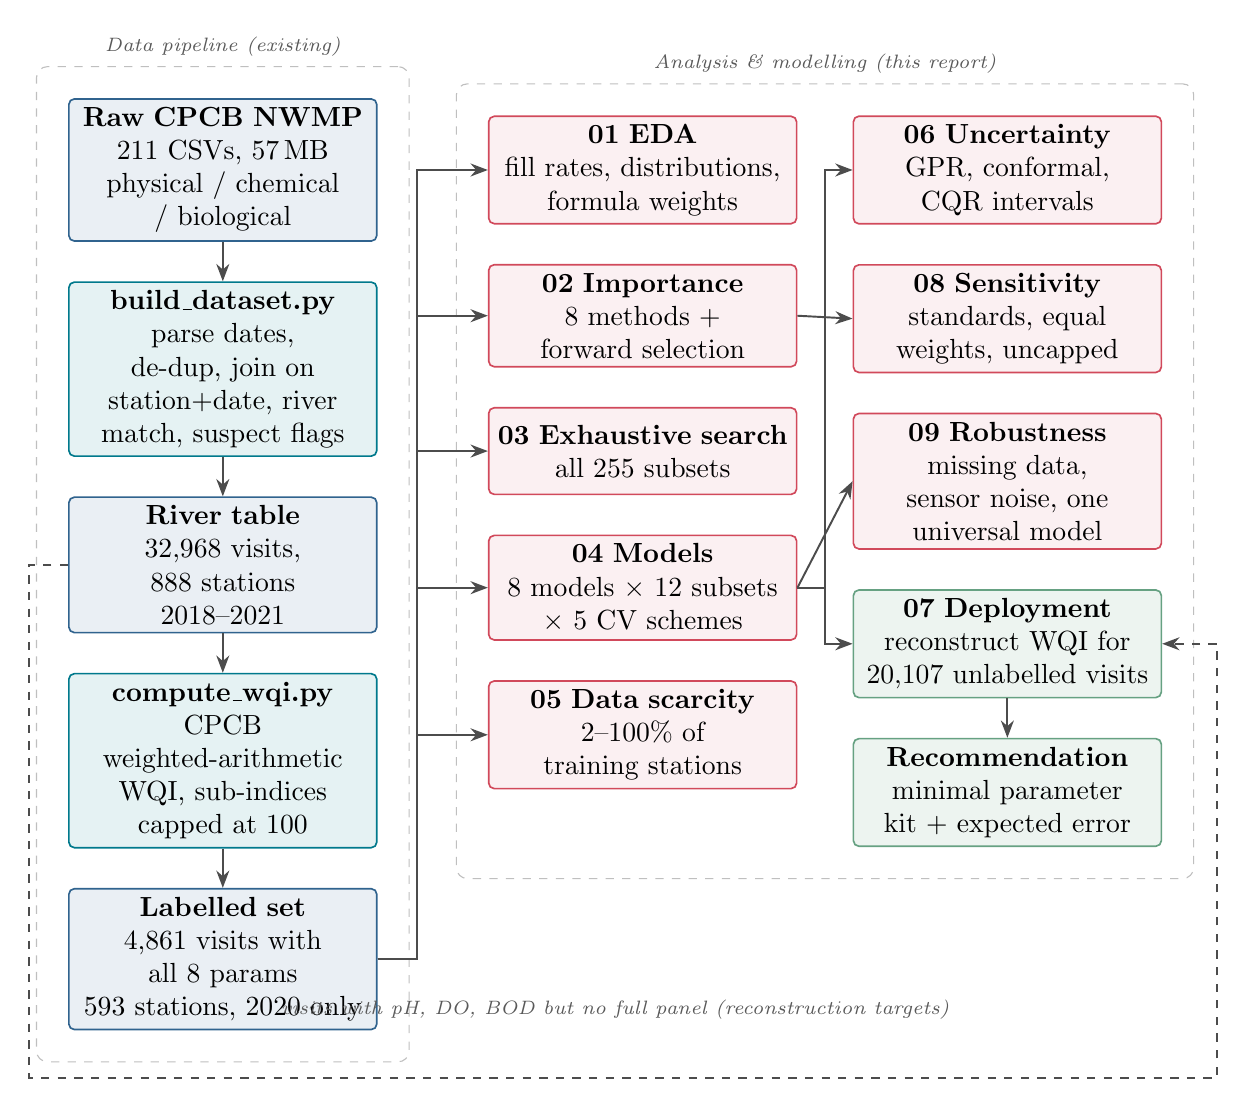
\begin{tikzpicture}[
  node distance=5mm and 7mm,
  box/.style={draw, rounded corners=2pt, align=center, minimum height=11mm, text width=37mm, inner sep=3pt, line width=0.6pt},
  data/.style={box, fill=c1!10, draw=c1},
  proc/.style={box, fill=c2!10, draw=c2},
  exp/.style={box, fill=c3!8, draw=c3},
  res/.style={box, fill=c5!12, draw=c5},
  arr/.style={-{Stealth[length=2.2mm]}, line width=0.7pt, draw=black!70},
  lab/.style={font=\scriptsize\itshape, text=black!65}
]
% stage 1: data
\node[data] (raw) {\textbf{Raw CPCB NWMP}\\211 CSVs, 57\,MB\\physical / chemical / biological};
\node[proc, below=of raw] (build) {\textbf{build\_dataset.py}\\parse dates, de-dup, join on station+date, river match, suspect flags};
\node[data, below=of build] (river) {\textbf{River table}\\32{,}968 visits, 888 stations\\2018--2021};
\node[proc, below=of river] (wqi) {\textbf{compute\_wqi.py}\\CPCB weighted-arithmetic WQI, sub-indices capped at 100};
\node[data, below=of wqi] (lab) {\textbf{Labelled set}\\4{,}861 visits with all 8 params\\593 stations, 2020 only};

% stage 2: analysis
\node[exp, right=14mm of raw] (eda) {\textbf{01 EDA}\\fill rates, distributions, formula weights};
\node[exp, below=of eda] (imp) {\textbf{02 Importance}\\8 methods + forward selection};
\node[exp, below=of imp] (comb) {\textbf{03 Exhaustive search}\\all 255 subsets};
\node[exp, below=of comb] (mod) {\textbf{04 Models}\\8 models $\times$ 12 subsets $\times$ 5 CV schemes};
\node[exp, below=of mod] (scar) {\textbf{05 Data scarcity}\\2--100\% of training stations};

\node[exp, right=7mm of eda] (unc) {\textbf{06 Uncertainty}\\GPR, conformal, CQR intervals};
\node[exp, below=of unc] (sens) {\textbf{08 Sensitivity}\\standards, equal weights, uncapped};
\node[exp, below=of sens] (rob) {\textbf{09 Robustness}\\missing data, sensor noise, one universal model};
\node[res, below=of rob] (dep) {\textbf{07 Deployment}\\reconstruct WQI for 20{,}107 unlabelled visits};
\node[res, below=of dep] (rec) {\textbf{Recommendation}\\minimal parameter kit + expected error};

\draw[arr] (raw) -- (build);
\draw[arr] (build) -- (river);
\draw[arr] (river) -- (wqi);
\draw[arr] (wqi) -- (lab);
\draw[arr] (lab.east) -- ++(5mm,0) |- (eda.west);
\draw[arr] (lab.east) -- ++(5mm,0) |- (imp.west);
\draw[arr] (lab.east) -- ++(5mm,0) |- (comb.west);
\draw[arr] (lab.east) -- ++(5mm,0) |- (mod.west);
\draw[arr] (lab.east) -- ++(5mm,0) |- (scar.west);
\draw[arr] (imp.east) -- (sens.west);
\draw[arr] (mod.east) -- ++(3.5mm,0) |- (unc.west);
\draw[arr] (mod.east) -- (rob.west);
\draw[arr] (mod.east) -- ++(3.5mm,0) |- (dep.west);
\draw[arr] (dep) -- (rec);
\draw[arr, dashed] (river.west) -- ++(-5mm,0) |- ($(lab.south)+(0,-6mm)$) -| ($(dep.east)+(7mm,0)$) -- (dep.east) node[pos=0, below, lab, xshift=-60mm, yshift=-1mm] {};
\node[lab] at ($(lab.south)!0.5!(rec.south)+(0,-9mm)$) {visits with pH, DO, BOD but no full panel (reconstruction targets)};

\begin{scope}[on background layer]
  \node[fit=(raw)(lab), draw=black!25, dashed, rounded corners, inner sep=4mm, label={[lab]above:Data pipeline (existing)}] {};
  \node[fit=(eda)(scar)(unc)(rec), draw=black!25, dashed, rounded corners, inner sep=4mm, label={[lab]above:Analysis \& modelling (this report)}] {};
\end{scope}
\end{tikzpicture}
\end{document}
